%%%%%%%%%%%%%%%%%%%%%%%%%%%%%%%%%%%%%%%%%%%%%%%%%%%%%%%%%%%%%%%%%%%%%%%%%%%%%%%%%%%%%
% uSIM2020_paper_format_guide.tex
% Base on a template kindly shared by the Building Simulation and Optimization 
% conference committee (BSO2020, IBSPA-England).
%%%%%%%%%%%%%%%%%%%%%%%%%%%%%%%%%%%%%%%%%%%%%%%%%%%%%%%%%%%%%%%%%%%%%%%%%%%%%%%%%%%%%

\documentclass[twocolumn, a4paper,10pt]{article}
\usepackage{boxedminipage}
\usepackage{nopageno}
\usepackage{graphicx}
\usepackage{natbib}
\usepackage{enumitem}
\usepackage[font=it]{caption}
\usepackage{hyperref}
\usepackage[usenames,dvipsnames]{xcolor}
\usepackage{listings}
\usepackage{caption}
\usepackage{subcaption}
\usepackage{tabularx,ragged2e,booktabs}

\usepackage[top=2.5cm, bottom=2.5cm, left=2.0cm, right=2.0cm,
columnsep=0.8cm]{geometry}

\setlength{\abovecaptionskip}{0.2cm}
\setlength{\belowcaptionskip}{0cm}
\setlength{\parindent}{0pt}

% Comment this line if you want to compile the paper without comments
\newcommand{\displaycomments}

\setcounter{secnumdepth}{-1}

%%%%%%%%%%%%%%%%%%%%%%%%%%%%%%%%%%%%%%%%%%%%%%%%%%%%%%%%%%%%%%%%%%%%%%%%%%%%%%%%%%%%%%%%%%%%%%%%%%%%%%%%%%%%%%%%%%%%%%%%%%%%%%%%%%%%
% Set fonts for title, section and subsection headings
\makeatletter
\renewcommand\title[1]{\gdef\@title{\fontsize{12pt}{2pt}\bfseries{#1}}}
\makeatletter
\renewcommand\section{\@startsection{section}{1}{\z@}{0.25cm}{0.1cm}{\normalfont\large\bfseries}}
% \normalfont\large
\makeatletter
\renewcommand\subsection{\@startsection{subsection}{1}{\z@}{0.2cm}{0.1cm}{\normalfont\normalsize\bfseries}}
\makeatletter
\renewcommand\subsubsection{\@startsection{subsection}{1}{\z@}{0.2cm}{0.1cm}{\normalfont\normalsize\itshape}}

\renewcommand\refname{References}


%%%%%%%%%%%%%%%%%%%%%%%%%%%%%%%%%%%%%%%%%%%%%%%%%%%%%%%%%%%%%%%%%%%%%%%%%%%%%%%%%%%%%%%
%%Configurations from the "enumitem" package to set the configurations
%%for the lists and remove undesired horizontal space for the enumerate
%%%%%%%%%%%%%%%%%%%%%%%%%%%%%%%%%%%%%%%%%%%%%%%%%%%%%%%%%%%%%%%%%%%%%%%%%%%%%%%%%%%%%%%
\setlist{itemsep=-0.1cm,topsep=0.1cm,labelsep=0.3cm}
\setenumerate{leftmargin=*}
%%%%%%%%%%%%%%%%%%%%%%%%%%%%%%%%%%%%%%%%%%%%%%%%%%%%%%%%%%%%%%%%%%%%%%%%%%%%%%%%%%%%%%%%
%%% END OF THE SETUP
%%%%%%%%%%%%%%%%%%%%%%%%%%%%%%%%%%%%%%%%%%%%%%%%%%%%%%%%%%%%%%%%%%%%%%%%%%%%%%%%%%%%%%%%



%%--------------------------------
% Custom configurations
\usepackage{tabu}
\usepackage{booktabs}
\usepackage{multirow}
\usepackage{amsmath, amssymb}
\usepackage{color}
\usepackage{url}
\usepackage{tikz}
\usepackage{pgfplots}
\usepackage{textgreek}

\pgfplotsset{compat=1.16}
\newtheorem{defn}{Definition}[section]
\newtheorem{rema}[defn]{Remark}
%QED box, from the TeXbook, p. 106. ----------------------------------
\newcommand\qed{{\unskip\nobreak\hfil\penalty50\hskip2em\vadjust{}
    \nobreak\hfil$\Box$\parfillskip=0pt\finalhyphendemerits=0\par}}

\renewcommand{\Re}{{\mathbb R}}
\newcommand{\Rep}{{\Re_{+}}}
\newcommand{\Na}{{\mathbb N}}
\newcommand{\Z}{{\mathbb Z}}
\newcommand{\codi}[2]{{\mathcal{C}^{#1}(#2)}}

\DeclareMathOperator{\sgn}{sgn}

%%%%%%%%%%%%%%%%%%%%%%%%%%%%%%%%%%%%%%%%%%%%%%%%%%
% see: http://mirror.aarnet.edu.au/pub/CTAN/macros/latex/contrib/listings/listings-1.3.pdf
\lstset{%
  basicstyle=\fontsize{8}{9}\selectfont\ttfamily,
%  basicstyle=\small, % print whole listing small
  keywordstyle=\color{red},
  identifierstyle=, % nothing happens
  commentstyle=\color{blue}, % white comments
  stringstyle=\color{OliveGreen}\it, % typewriter type for strings
  showstringspaces=false,
  numbers=left,
  numberstyle=\tiny,
  numbersep=5pt} % no special string space
%%%%%%%%%%%%%%%%%%%%%%%%%%%%%%%%%%%%%%%%%%%%%%%%%%
\lstdefinelanguage{Modelica}{%
  morekeywords={Modelica,Thermal,HeatTransfer,Interfaces, flow, %
    SI,Temperature,HeatFlowRate,HeatPort, Real, zeros},
  sensitive=false,
  morecomment=[l]{//},
  morecomment=[s]{/*}{*/},
  morestring=[b]",
  emph={equation, partial, connector, model, public, end, %
    extends, parameter}, emphstyle=\color{blue},
}
%%%%%%%%%%%%%%%%%%%%%%%%%%%%%%%%%%%%%%%%%%%%%%%%%%


%%% Please keep the \vspace{-1.5cm} at the top
\title{%
Short-term Forecasting of Building Level Electricity Demand in Findhorn,\\	% Line 1
%%% Please keep the \vspace{4pt} between lines in the title
\vspace{4pt}
Scotland Using CNN-LSTM Architecture % Line 2 - If there is no second line then just put \phantom{Line 2} here
}

%%% Change or delete text before "\\" on the lines below to keep the layout but don't remove the "\\"
%%% Do not exceed more than 6 lines for authors and affiliations
\author{
Ashkan Lotifipoor$^1$, Sandhya Patidar$^2$, David Jenkins$^2$\\ % Line 4
$^1$PhD researcher, Institute for Infrastructure and Environment, Heriot-Watt University\\ % Line 5
$^2$Associate Professor, Institute for Infrastructure and Environment, Heriot-Watt University\\ % Line 6
\\ % Line 7
\\ % Line 8
} % Line 9 - Last line
\date{\vspace{-0.5cm}}	% remove default date and replace the Blank 10th line

\begin{document}

\maketitle

\section*{Abstract}	% Section headings need to be upper and lower case.
\addtocounter{section}{1}
An accurate forecasting of energy demand could serve several purposes including optimising the utilisation of available resources and identification of any potential risks, which is essential for developing effective management and planning strategies/policies for a robust and resilient energy system. This paper is aimed to develop a novel deep learning based energy demand prediction model by utilising the combination of Convolutional neural networks and Long Short-term Memory units. The proposed model consist of two one dimensional convolutional layer with max pooling, two bidirectional LSTM layers and finally three fully connected dense layer. The energy consumption data available for a household based in Findhorn ecovillage located in the north of Scotland for a six-week period during the February and March of 2015 was utilised to train, validate, and test the models. The proposed model provides energy demand prediction for short-term forecasting (5 minute). The results obtained from the model are compared against four of the classical and widely applied algorithms for time series forecasting: autoregressive integrated moving average (ARIMA), light gradient boosting machine (LightGBM), random forest (RF), and deep neural networks (DNN). The RMSE value on the test data was significantly lower that other algorithms.

\section*{Introduction}
During the past decade smart meters and grids have become widespread around the globe, for example, the numbers of smart meters installed in the UK reached 14.9 million at end of June 2019 \citep{RN1251}. Smart meters provide information on supply and demand, and equip researchers and industry stake-holders with a vast amount of energy consumption data for demand analytics. 

Over the years, researchers have used this data to improve energy efficiency and sustainability in many frontier, such as community energy modelling, energy management and energy forecasting. An accurate forecasting of energy demand could serve several purposes including optimising the utilisation of available resources and identification of any potential risks, which is essential for developing effective management and planning strategies/policies for a robust and resilient energy system. ASHRAE breaks energy estimation models into two main categories: physics-based and data-driven models \citep{RN1250}. Data-driven models basically divides into two methodologies, a statistical model or a machine learning algorithm.

In recent years, with artificial intelligence boom and the widespread use of machine learning algorithms in various fields, many researcher has used these techniques for accurate forecasting of energy demand. 

\cite{RN21} in a comprehensive study, evaluate the performance of linear regressor, RBF kernel support vector regressor (SVR), adaboost regressor, bagging regressor, gradient boosting regressor, random forest, multi-layer perceptron regressor (MLP regressor), and K-nearest neighbor regressor among other models. \cite{RN1199} studied the performance of Support Vector Machine (SVM) and Recurrent Neural Networks on the day-ahead electricity consumption prediction of a population of households. The training of the models was performed with observed weather data while the actual forecast was performed using predicted weather data. \cite{RN1194} compared three algorithms, namely Random Forest, K-nearest neighbour, Linear Regressor, for forecasting urban area electrical energy demand. Similarly, \cite{RN1197} used XGboost, Extreme learning machine (ELM) and MLP for energy demand prediction for residential buildings.

The deep learning has also drawn the attention of many researcher in this area. \cite{RN13} investigated the effectiveness of using Convolutional Neural Networks (CNN) for performing energy load forecasting at individual building level. \cite{RN29} compared the performance of MLPs with SVMs, Gaussian Processes, Regression Trees, Ensemble Boosting and Linear Regression. \cite{RN1195} provided a review of using deep learning with state explainable autoencoder for electric energy consumption prediction. The developed model consists of a projector and a predictor, similar to an auto-encoder consisting of an encoder and a decoder. \cite{RN59} explored the usage of MLP for the medium, short and very short-term forecasting of load demand. Human thermal comfort-discomfort biometeorological index was used as one of the features in forecasting.

This paper is aimed to develop a novel deep learning based energy demand prediction model by utilising the potentials of convolutional neural networks and Long short-term memory (LSTM) units. The proposed model provides EDP for short-term forecasting (5 minute). The results obtained from the model are compared against four of the classical and widely applied algorithms: autoregressive integrated moving average (ARIMA), random forest, light gradient boosting machine (LightGBM), and deep neural networks (DNN). The remaining of the paper is organised as follows: Study area and data collection section presents details about the dataset; Methodology Section introduces the different elements of the methodology; next section reports the results of the methodology and baseline models on dataset and last section provides conclusions and ideas for future works.

\section*{Study Area and Data Collection}
To train and test the developed models, high resolution data gathered from the Findhorn Ecovillage site, located in northern Scotland, is used in this study. The demand data of Findhorn was collected as part of the UK National Centre for Energy System Integration (CESI) project. For the case study, high resolution data (five minute interval) collected over a continuous time-period from February 2015 to March 2015 is used.

\begin{figure}[ht]
    \centering
    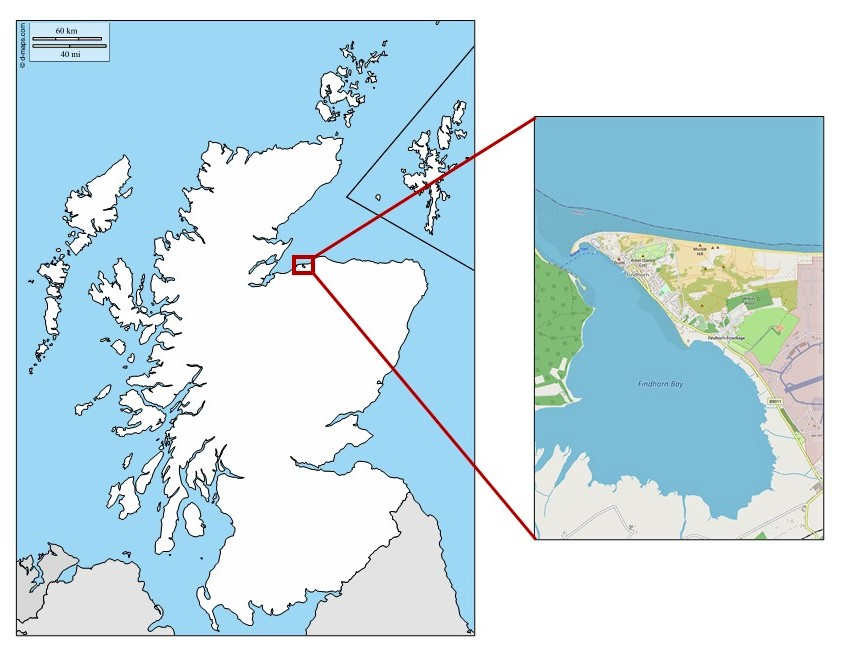
\includegraphics[scale=0.28]{img/Finhorn_Postion.jpg}
    \caption{Findhorn Ecovillage Position in Scotland}
    \label{fig:Finhorn_Postion}
\end{figure}

The selected household for this study is built in 2 floors with an area of 96 m\textsuperscript{2}. The reading from the smart meter is soley related to electricity usage, as the house uses a gas boiler for heating purposes. The graph for the building demand can be seen in Figure 2.

\begin{figure}[ht]
    \centering
    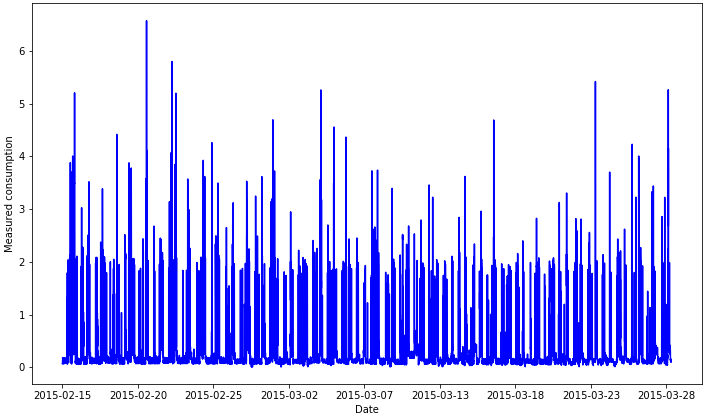
\includegraphics[scale=0.3]{img/edp_graph.png}
    \caption{Demand graph from Feb 2015 to Mar 2015}
    \label{fig:edp_graph}
\end{figure}

\section*{Methodology}

\subsection*{Deep Neural Networks}

Perceptrons were developed in the 1950s and 1960s by \cite{RN1279}, inspired by earlier work by \cite{RN1280}. A perceptron takes in some number of inputs, x\textsubscript{1}, x\textsubscript{2}, . . . , x\textsubscript{n}, each of which is multiplied by a specific weight, w\textsubscript{1}, w\textsubscript{2}, . . . , w\textsubscript{n}. These weighted inputs are, summed together to produce the logit of the neuron. The logit is then passed through a linear function to produce the output \citep{RN1281}. In order to learn complex relationships, we need to use neurons that employ some sort of nonlinearity. Today, it's more common to use other types of neurons, namely the sigmoid neuron. Sigmoid neuron is similar to a perceptron, except that the output is not 0 or 1. Instead, it's \( \sigma (w⋅x+b) \), where \( \sigma\) is a sigmoid function.

A standard neural network consists of many neurons, each producing a sequence of real-valued activation. Many researchers had wanted for decades to train deep multi-layer neural networks, but no successful attempts were reported before 2006 \citep{RN1284}. Finaly, \cite{RN1285} at University of Toronto introduced Deep Belief Networks (DBNs) with a learning algorithm that greedily trains one layer at a time. Deep learning methods aim at learning feature hierarchies with features from higher levels of the hierarchy formed by the composition of lower level features \citep{RN1284}. Deep feedforward networks, also called feedforward neural networks, or multilayer perceptrons (MLPs), are the quintessential deep learning models \citep{RN1282}.

\subsubsection*{Convolutional Neural Networks}

Convolutional nets were inspired by the visual system’s structure. The first computational models based on these local connectivities between neurons and on hierarchically organised transformations of the image are found in \cite{RN1286}. Later, LeCun and collaborators designed and trained convolutional networks using the error gradient, obtaining state-of-the-art performance \citep{RN1287}.

Convolution preserves the relationship between pixels by learning image features using small squares of input data. It is a mathematical operation that takes two inputs such as image matrix and a filter.

The architecture of a CNN is designed to take advantage of the 2D structure of an input image. This is achieved with local connections and tied weights followed by some form of pooling which results in translation invariant features. 

Similarly to computer vision tasks, in time series problems it is desired to extract a small number of low level features with a small receptive fields across the entire input. This method can significantly improve the accuracy of prediction system while keeping the computation cost at an acceptable range.

\subsubsection*{Long Short-term Memory}

The most effective sequence models in deep learning are called gated recurrent neural networks. These include the long short-term memory (LSTM) and the gated recurrent units (GRU) \citep{RN1282}). In order to combat the problem of vanishing gradients \citep{RN1289}, \cite{RN1288} introduced the long short-term memory (LSTM) architecture by introducing self-loops to produce paths where the gradient can flow for long duration. A crucial addition has been to make the weight on this self-loop conditioned on the context, rather than fixed \citep{RN1290}.

LSTMs make small modifications to the information by multiplications and additions. With LSTMs, the information flows through a mechanism known as cell states. This way, LSTMs can selectively remember or forget things. Those gates act on the signals they receive, and similar to the neural network’s nodes, they block or pass on information based on its strength and import, which they filter with their own sets of weights. Those weights, like the weights that modulate input and hidden states, are adjusted via the recurrent networks learning process. That is, the cells learn when to allow data to enter, leave or be deleted through the iterative process of making guesses, backpropagating error, and adjusting weights via gradient descent \citep{RN1282}.

\begin{figure}[ht]
    \centering
    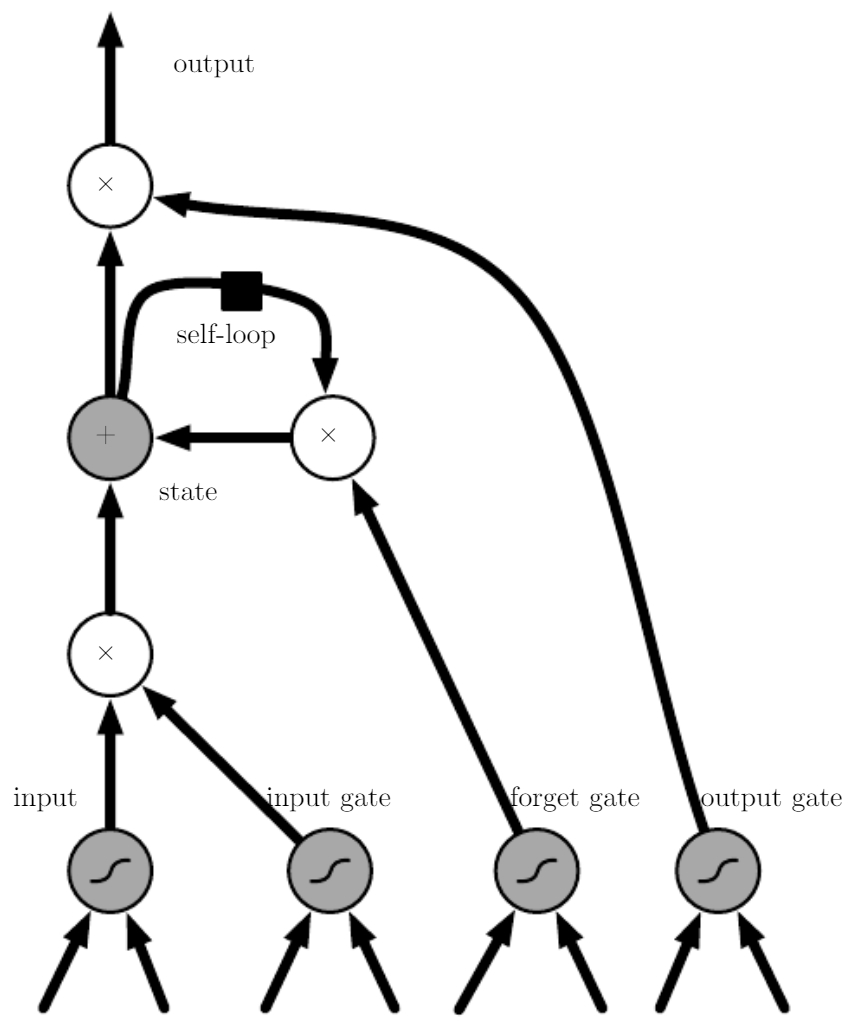
\includegraphics[scale=0.2]{img/lstm.jpg}
    \caption{LSTM Architecture \citep{RN1282}}
    \label{fig:lstm}
\end{figure}

\subsubsection*{Model Architecture}

Both CNNs and LSTMs have shown significant increase in performance over Deep Neural Networks (DNNs) across a variety of tasks. CNNs, LSTMs and DNNs are complementary in their modelling capabilities, as CNNs are good at reducing frequency variations, LSTMs are good at sequence modelling, and DNNs are appropriate
for mapping features to a more separable space \citep{RN1274}. In this paper, a deep neural net is developed which will use this complementarity to predict energy demand.

Figure 4 shows the complete architecture of the developed model. The two convolutional layer will extract features form the input variables (energy demand with 5 min interval). The convolutional layers develop a feature map of the input variables which will improve the accuracy of the model in comparison with vanilla LSTM networks. After each convolutional layer there is a max pooling layer which acts as a tool to reduce over-fitting and to minimise the computational cost by reducing the number of parameters to learn. Max pooling is a sample-based discretisation process and the objective is to down-sample an input representation and reducing its dimensionality \citep{RN1291}. By using a pooling layer in the architecture only features with highest value and importance will be selected. 

\begin{figure}[ht]
    \centering
    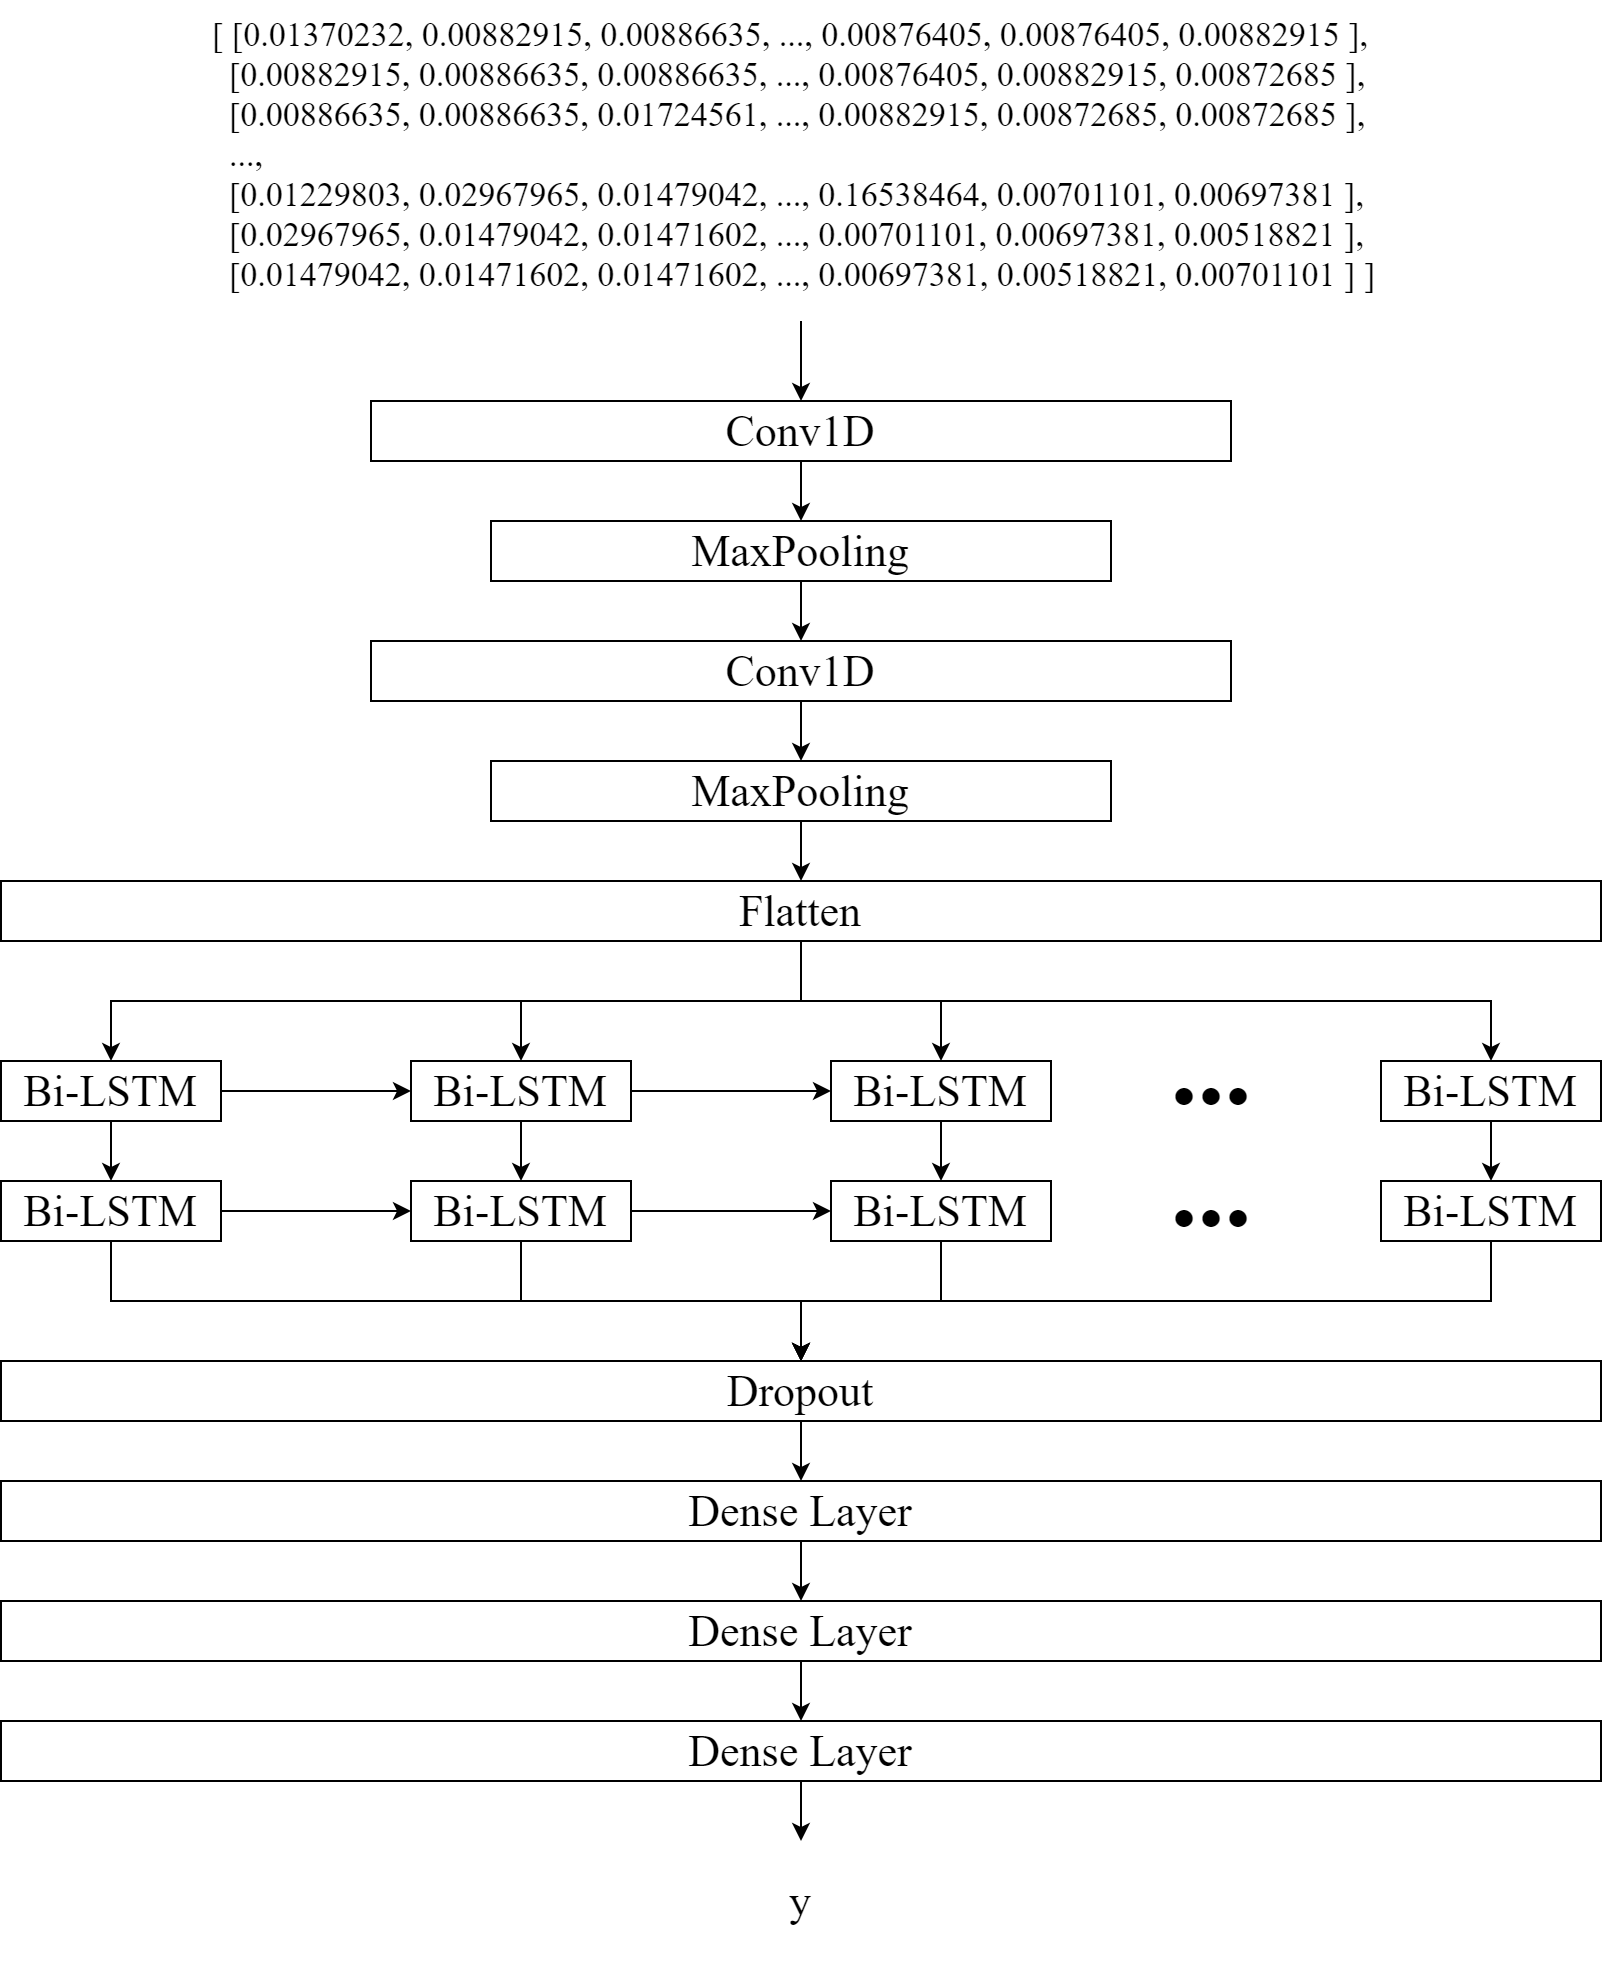
\includegraphics[scale=0.12]{img/architecture.png}
    \caption{CNN-LSTM Architecture}
    \label{fig:CNN-LSTM}
\end{figure}

After flattening the output of convolutional layers, the information is passed to the two Bi-LSTM layers to detect patterns in long periods of time in both direction. Finally, the output of the layers will pass onto the three fully-connected dense layers for making prediction.

The proposed methodology was implemented to perform prediction for next five minutes consumption. In order to do this, 35 previous observation was fed into the model as lagged features. This number was selected based on a grid search to obtain the optimum window size for maximising the performance and minimise the computation cost. For the CNN layers the filter size of 128 was selected as the optimum number with kernel size of 2. The activation function for these layers was the linear rectifier unit (ReLU) function which is the the default recommendation in modern neural networks \citep{RN1282}. As explained earlier for pooling phase of the network the max pooling was selected with pool size of 2. Once the CNN layers made their feature maps and it was flatten, their output was sent to two Bi-LSTM layers.

Bidirectional RNN are two independent RNNs together. This structure allows the networks to have both backward and forward information about the sequence at each time step. Bidirectional layers will run the inputs in two ways, one from past to future and one from future to past and what makes this method powerful is that it enables the network in any point in time to preserve information from both past and future. Based on our experiments, using this architecture help the model to better understand the patterns in the demand load. Next, for regularising the network a dropout layer with dropout rate of 0.3 was used after the second Bi-LSTM layer.

 In the developed model, three fully connected dense layer with 50, 10 and 1 neurons were used, respectively. These layers used the ReLU function as their activation function.  For compiling the model, Adaptive Moment Estimation (Adam) \citep{RN1292} algorithm was used as the gradient based optimiser. The value of learning rate was obtained by running the model first with a learning rate scheduler.
Mean square error (MSE) was used as the loss function for training the model and root mean square error (RMSE) and mean absolute error (MAE) were used as the metrics for evaluating the performance of the model. Furthermore, a early stopping method was used to prevent the model to overfit on the train data. the model was train 200 epochs with batch size of 256. In total, 1,385,275 parameters were trained during the model development phase. The model was developed using the Keras neural-network library with TensorFlow 2.1.0 backend in Python.

\subsubsection*{Evaluation index of model performances}

The predicted values by the proposed model are evaluated by three performance metrics for regression models, MAE, MSE and RMSE. Furthermore, the residual error was calculated for test data to evaluate the performance of the model by plotting its distribution. In regression analysis, the difference between the observed value of the dependent variable ($y_{i}$) and the predicted value ($x_{i}$) is called the residual error (e).
% $$  e = y - \hat{y} $$
$$ e = y_{i} - x_{i} $$

MAE measures the average magnitude of the errors in predicted values, without considering their direction. The MAE is a linear score which means that all the individual differences are weighted equally in the average. MAE is calculated as follows.

$$ MAE = \frac{1}{n}\sum_{i=1}^{n}abs(y_{i} - x_{i}) $$

MSE  measures the average of the squares of the errors. In other words, it is the average squared difference between the predicted values and the actual values. The equation for MSE is as follows.

$$ MSE = \frac{1}{n}\sum_{i=1}^{n}(y_{i} - x_{i})^{2} $$

RMSE is the standard deviation of the residual errors. It is the square root of the average of squared differences between predictions and actual values. The RMSE is calculated as:

$$ RMSE = \sqrt{(\frac{1}{n})\sum_{i=1}^{n}(y_{i} - x_{i})^{2}} $$


\section*{Results and Discussion}

The performance of the developed network is evaluated against one mainstream statistical method (ARIMA) and three established machine learning algorithms, namely Random Forest, Light Gradient Boosting Machine (LightGBM) \citep{RN1293} and a DNN. LightGBM is a gradient boosting framework that uses tree based learning algorithms. For the ARIMA model the hyperparameters values (p, d, q) were chosen by using autocorrelation function (ACF) and passive autocorrelation function (PACF).

For Random Forest and LightGBM model, the hyperparameters were tuned by performing grid searche so that the maximum performance of the individual models are achieved. Moreover, cross validation was performed to check the degree of generalisation of the models. For the DNN, similar values and hyperparameters (Activation function = ReLU, Optimisation algorithm = Adam with learning rate of 1e-4) were used. All models used the same 80/20 ratio for splitting the dataset for training and testing, however, the train/validation/test split was used in the neural networks (20\% of train data was used for validation). Table \ref{tab:tabel1} summaries the results (MAE, MSE and RMSE) obtained from all the algorithms for training and testing sets.

\begin{table*}[ht]
        \caption{Performance of different algorithms on the dataset}
        \centering
        \setlength{\tabcolsep}{4pt}
        \begin{tabularx}{\textwidth}{>{\hsize=1.9\hsize\bfseries\RaggedRight}X!{\extracolsep{\fill}}*{12}{>{\centering\arraybackslash\hsize=0.48\hsize}X}}
                \toprule[1pt]\midrule[0.3pt]
                \multicolumn{13}{c}{\textbf{Evaluation Results}} \\ \midrule[0.3pt]
                \textbf{}& \multicolumn{2}{c}{\textit{ARIMA}} & \multicolumn{2}{c}{\textit{Random Forest}} & \multicolumn{2}{c}{\textit{LightGBM}} & \multicolumn{2}{c}{\textit{DNN}} & \multicolumn{2}{c}{\textit{CNN-LSTM}} & \multicolumn{2}{c}{\textit{C24}} \\
                \cmidrule(lr){2-3} \cmidrule(lr){4-5} \cmidrule(lr){6-7} \cmidrule(lr){8-9} \cmidrule(lr){10-11} \cmidrule(lr){12-13}%
                {} & Train & Test & Train & Test & Train & Test & Train & Test & Train & Test & Train & Test \\
                \addlinespace%
                {MAE} & 0.230 & - & 0.207 & 0.205 & 0.245 & 0.276 & 0.202 & 0.201 & 0.200 & 0.192 & - & 0.180 \\
                \addlinespace%
                {MSE} & 0.227 & - & 0.200 & 0.298 & 0.154 & 0.225 & 0.211 & 0.209 & 0.206 & 0.214 & - & 0.151 \\
                \addlinespace%
                {RMSE} & 0.477 & - & 0.459 & 0.476 & 0.493 & 0.475 & 0.479 & 0.469 & 0.454 & 0.463 & - & 0.389 \\
                %\addlinespace
                %\midrule
                \midrule[0.3pt]\bottomrule[1pt]
        \end{tabularx}
        \label{tab:tabel1}
\end{table*}

Although the difference in performance of different models is not substantial, it can be seen that the CNN-LSTM network provides the lowest values in all three evaluation metrics for accurate forecast, outperforming all other models. DNNs require a large size training data because of the huge number of parameters needed to be tuned by a learning algorithm. The issue in DNN is that the network starts with a poor initial state and then an optimisation algorithm such as stochastic gradient descent or Adam is used to converge the network to an optimal position. So, given more data to the CNN-LSTM network it will surly outperform other model significantly.

In addition, it can be argued that the CNN-LSTM network can be generalised best to unseen data due to the low difference between RMSE for train and test data, which increase the robustness and generality of the model. The reason for this could be all the measures that were implemented to prevent the model from overfitting, such as the use of maxpooling layers, dropout layer, and early stopping. Furthermore, it is worth noting that all machine learning algorithms outperform the statistical model used in this study, showing substantial promise for the machine learning algorithms in time series forecasting of electricity demand load.

Figure \ref{fig:prediction} depicts a samples from CNN-LSTM network projections against the actual measurement in the testing set.It can be been that the CNN-LSTM is able to follow the general trend of data showing capabilities of generalisation. The superior generalisation capability of CNN-LSTM was also discussed earlier.

\begin{figure}[ht]
    \centering
    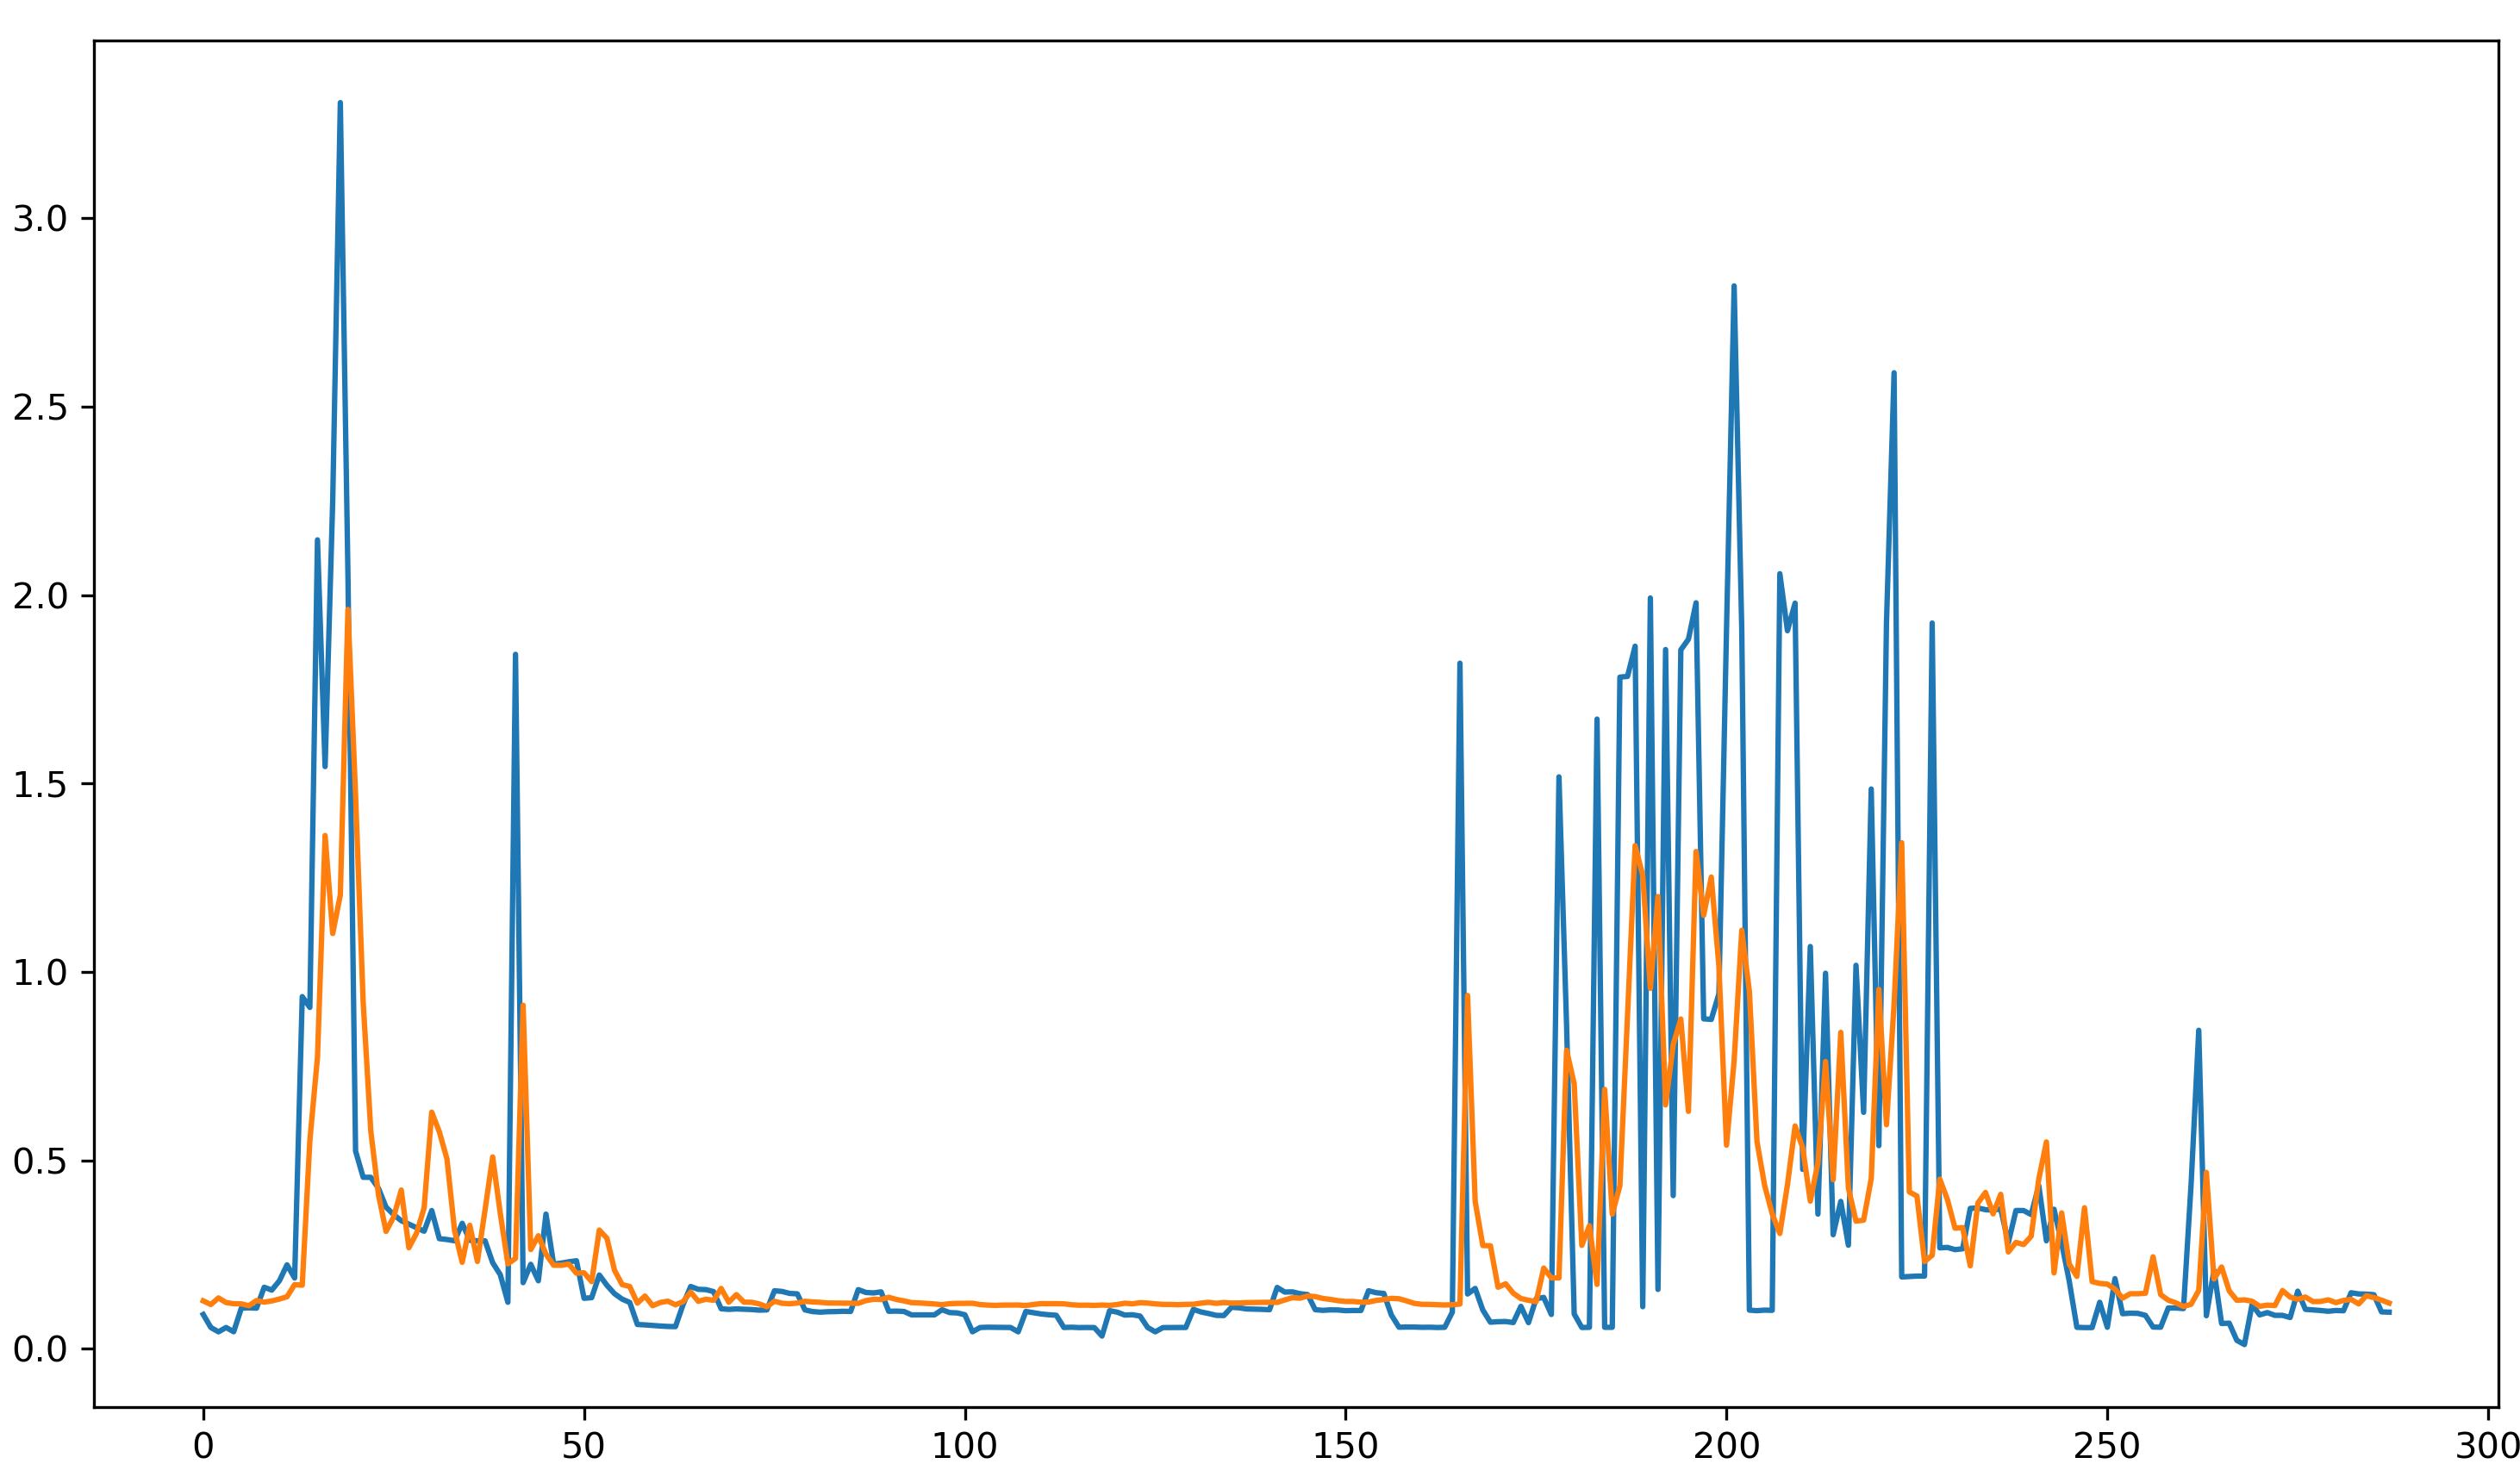
\includegraphics[scale=0.3]{img/test_day.png}
    \caption{Predicted values and actual values for a day}
    \label{fig:prediction}
\end{figure}

Although the most common metrics were used in order to assess the accuracy of models predictions, it is particularly difficult to conclude whether the predictions are consistently accurate or not. For this reason, the error probability density function is depicted in Figure \ref{fig:re_error}. Probability density functions that are closer to zero produce both accurate and reliable results.

\begin{figure}[ht]
    \centering
    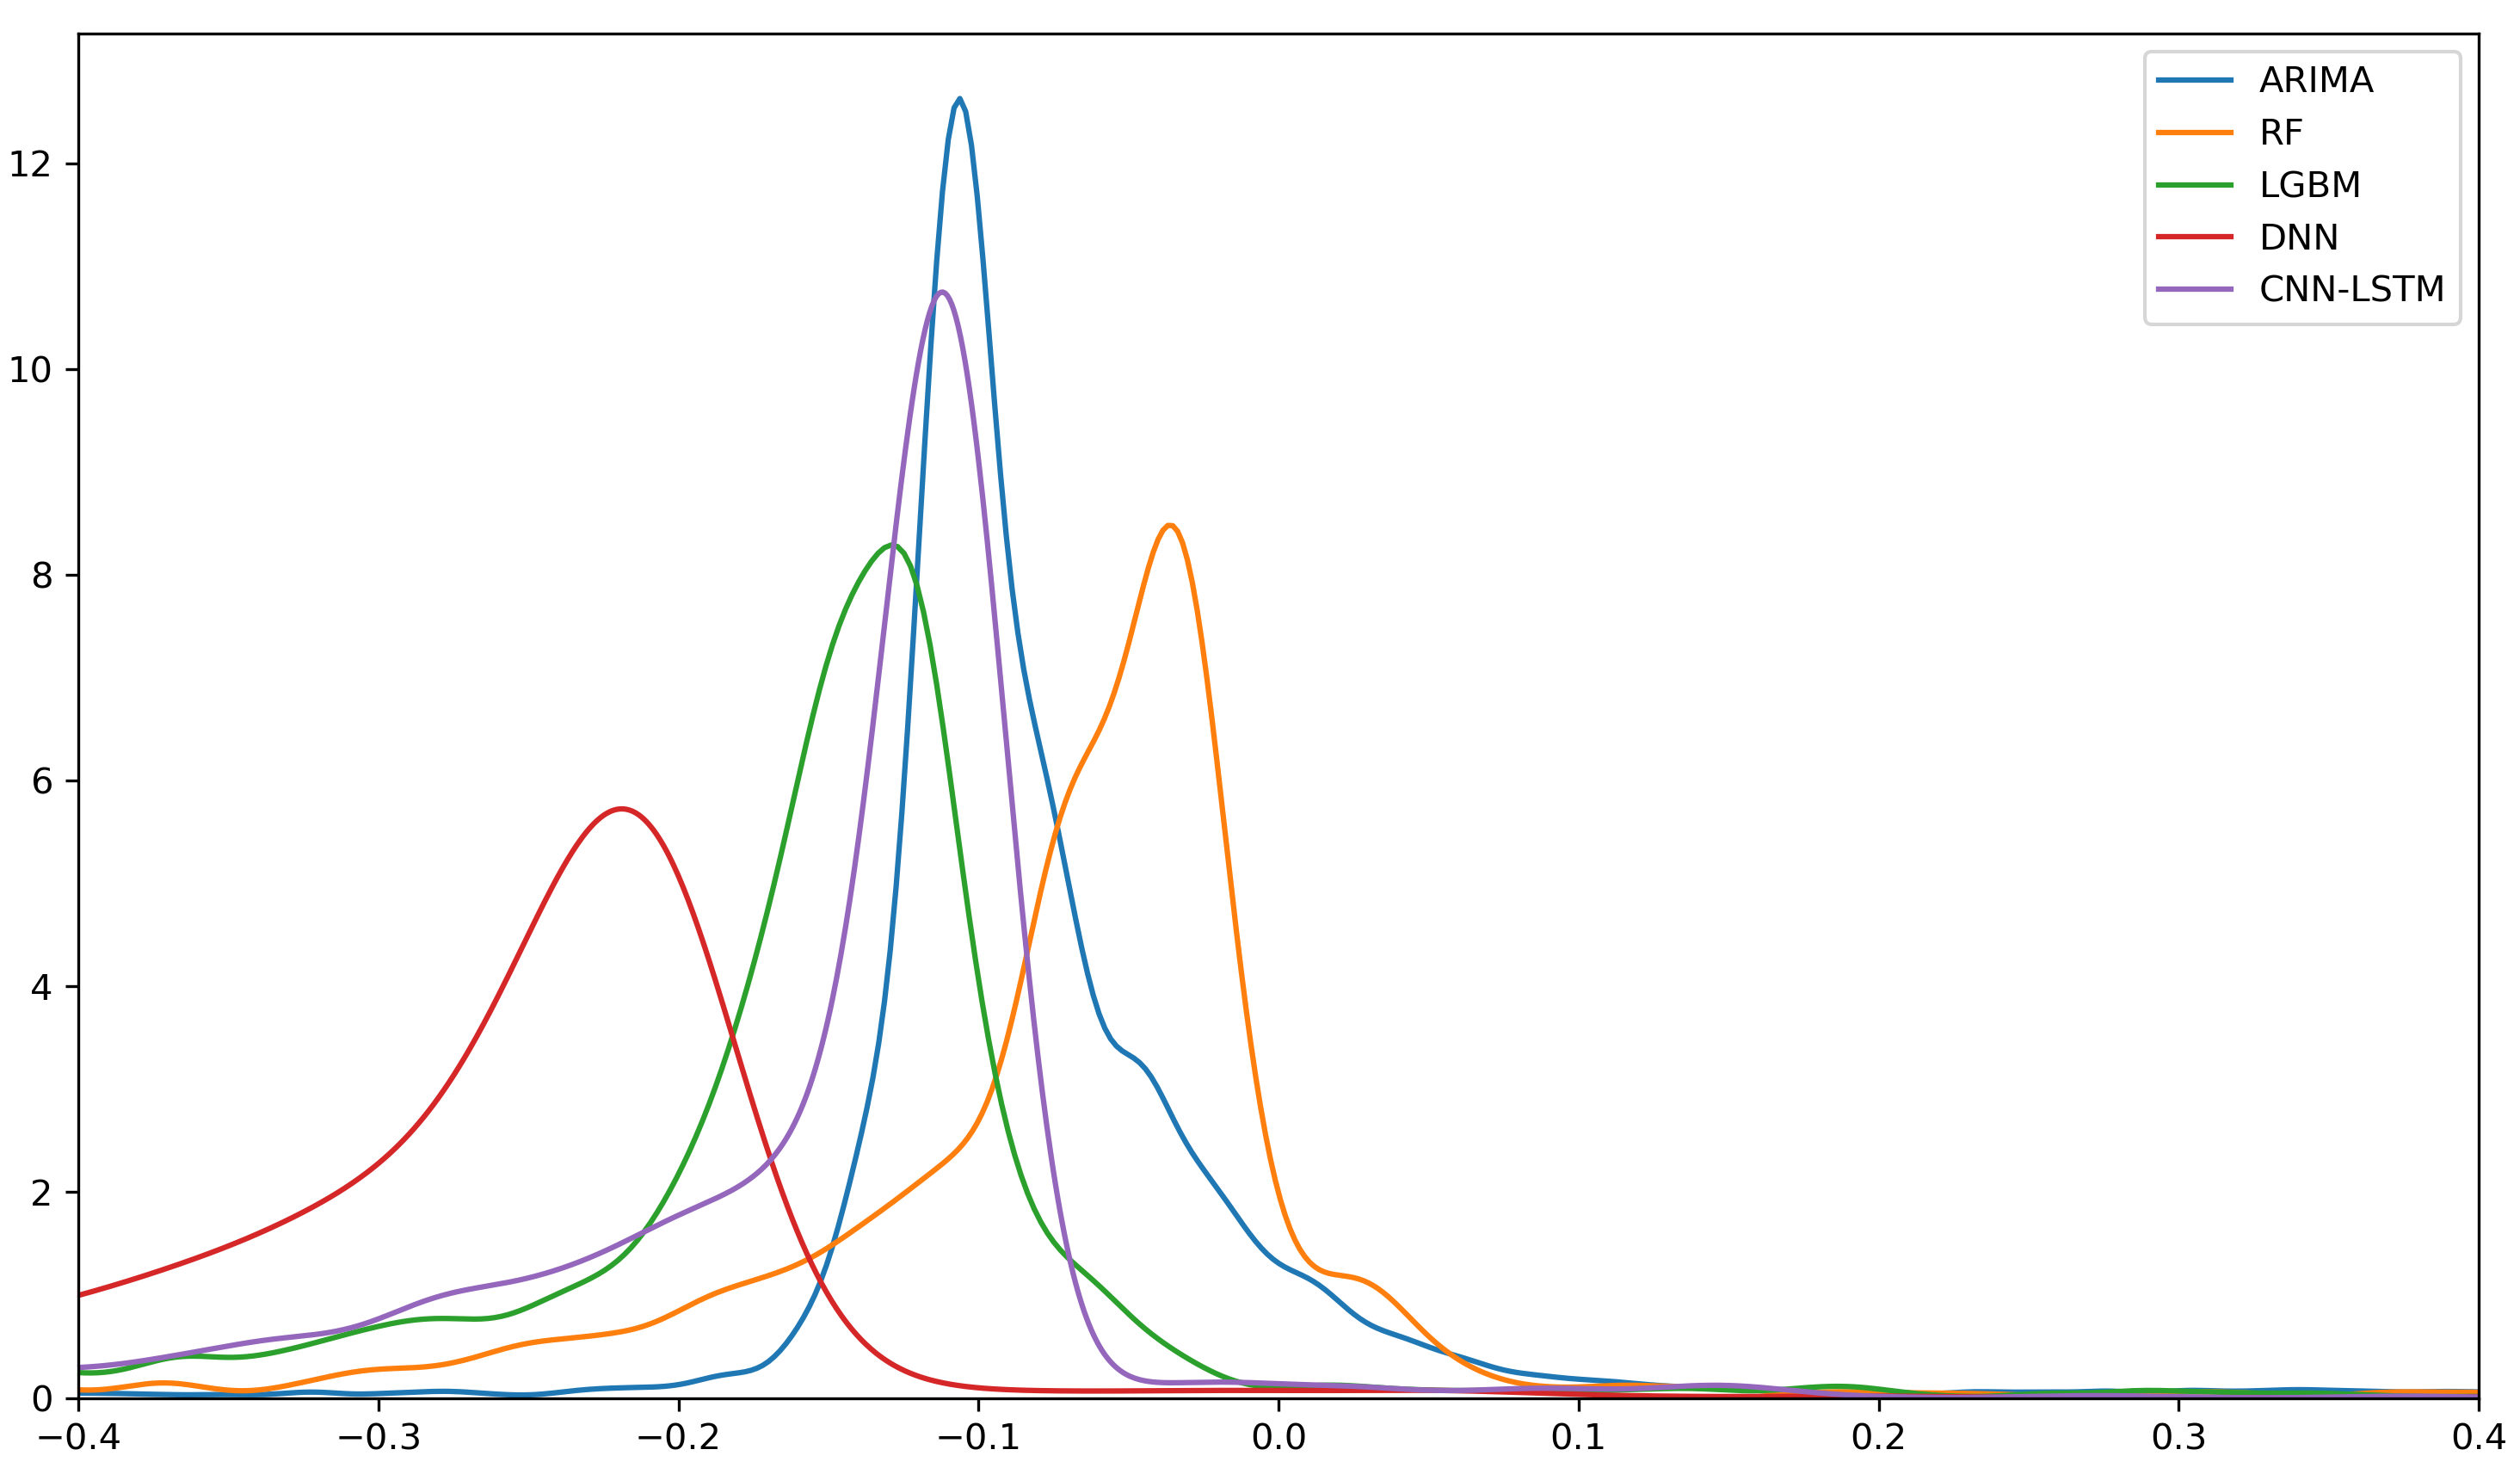
\includegraphics[scale=0.3]{img/pdf.png}
    \caption{Histogram of Residual Error on test data}
    \label{fig:re_error}
\end{figure}

Furthermore, as a mean to evaluate the develop model further, the prediction of unseen data from a different building in Findhorn village was selected for testing the model. It is worth noting that the chosen building has similar construction and overall design as the building used for training the model. The result shows (under C24 in Table 1) even better performance of developed model on this dataset. The proposed model predicted the demand for this building by RMSE value of 0.389.

\begin{figure}[ht]
    \centering
    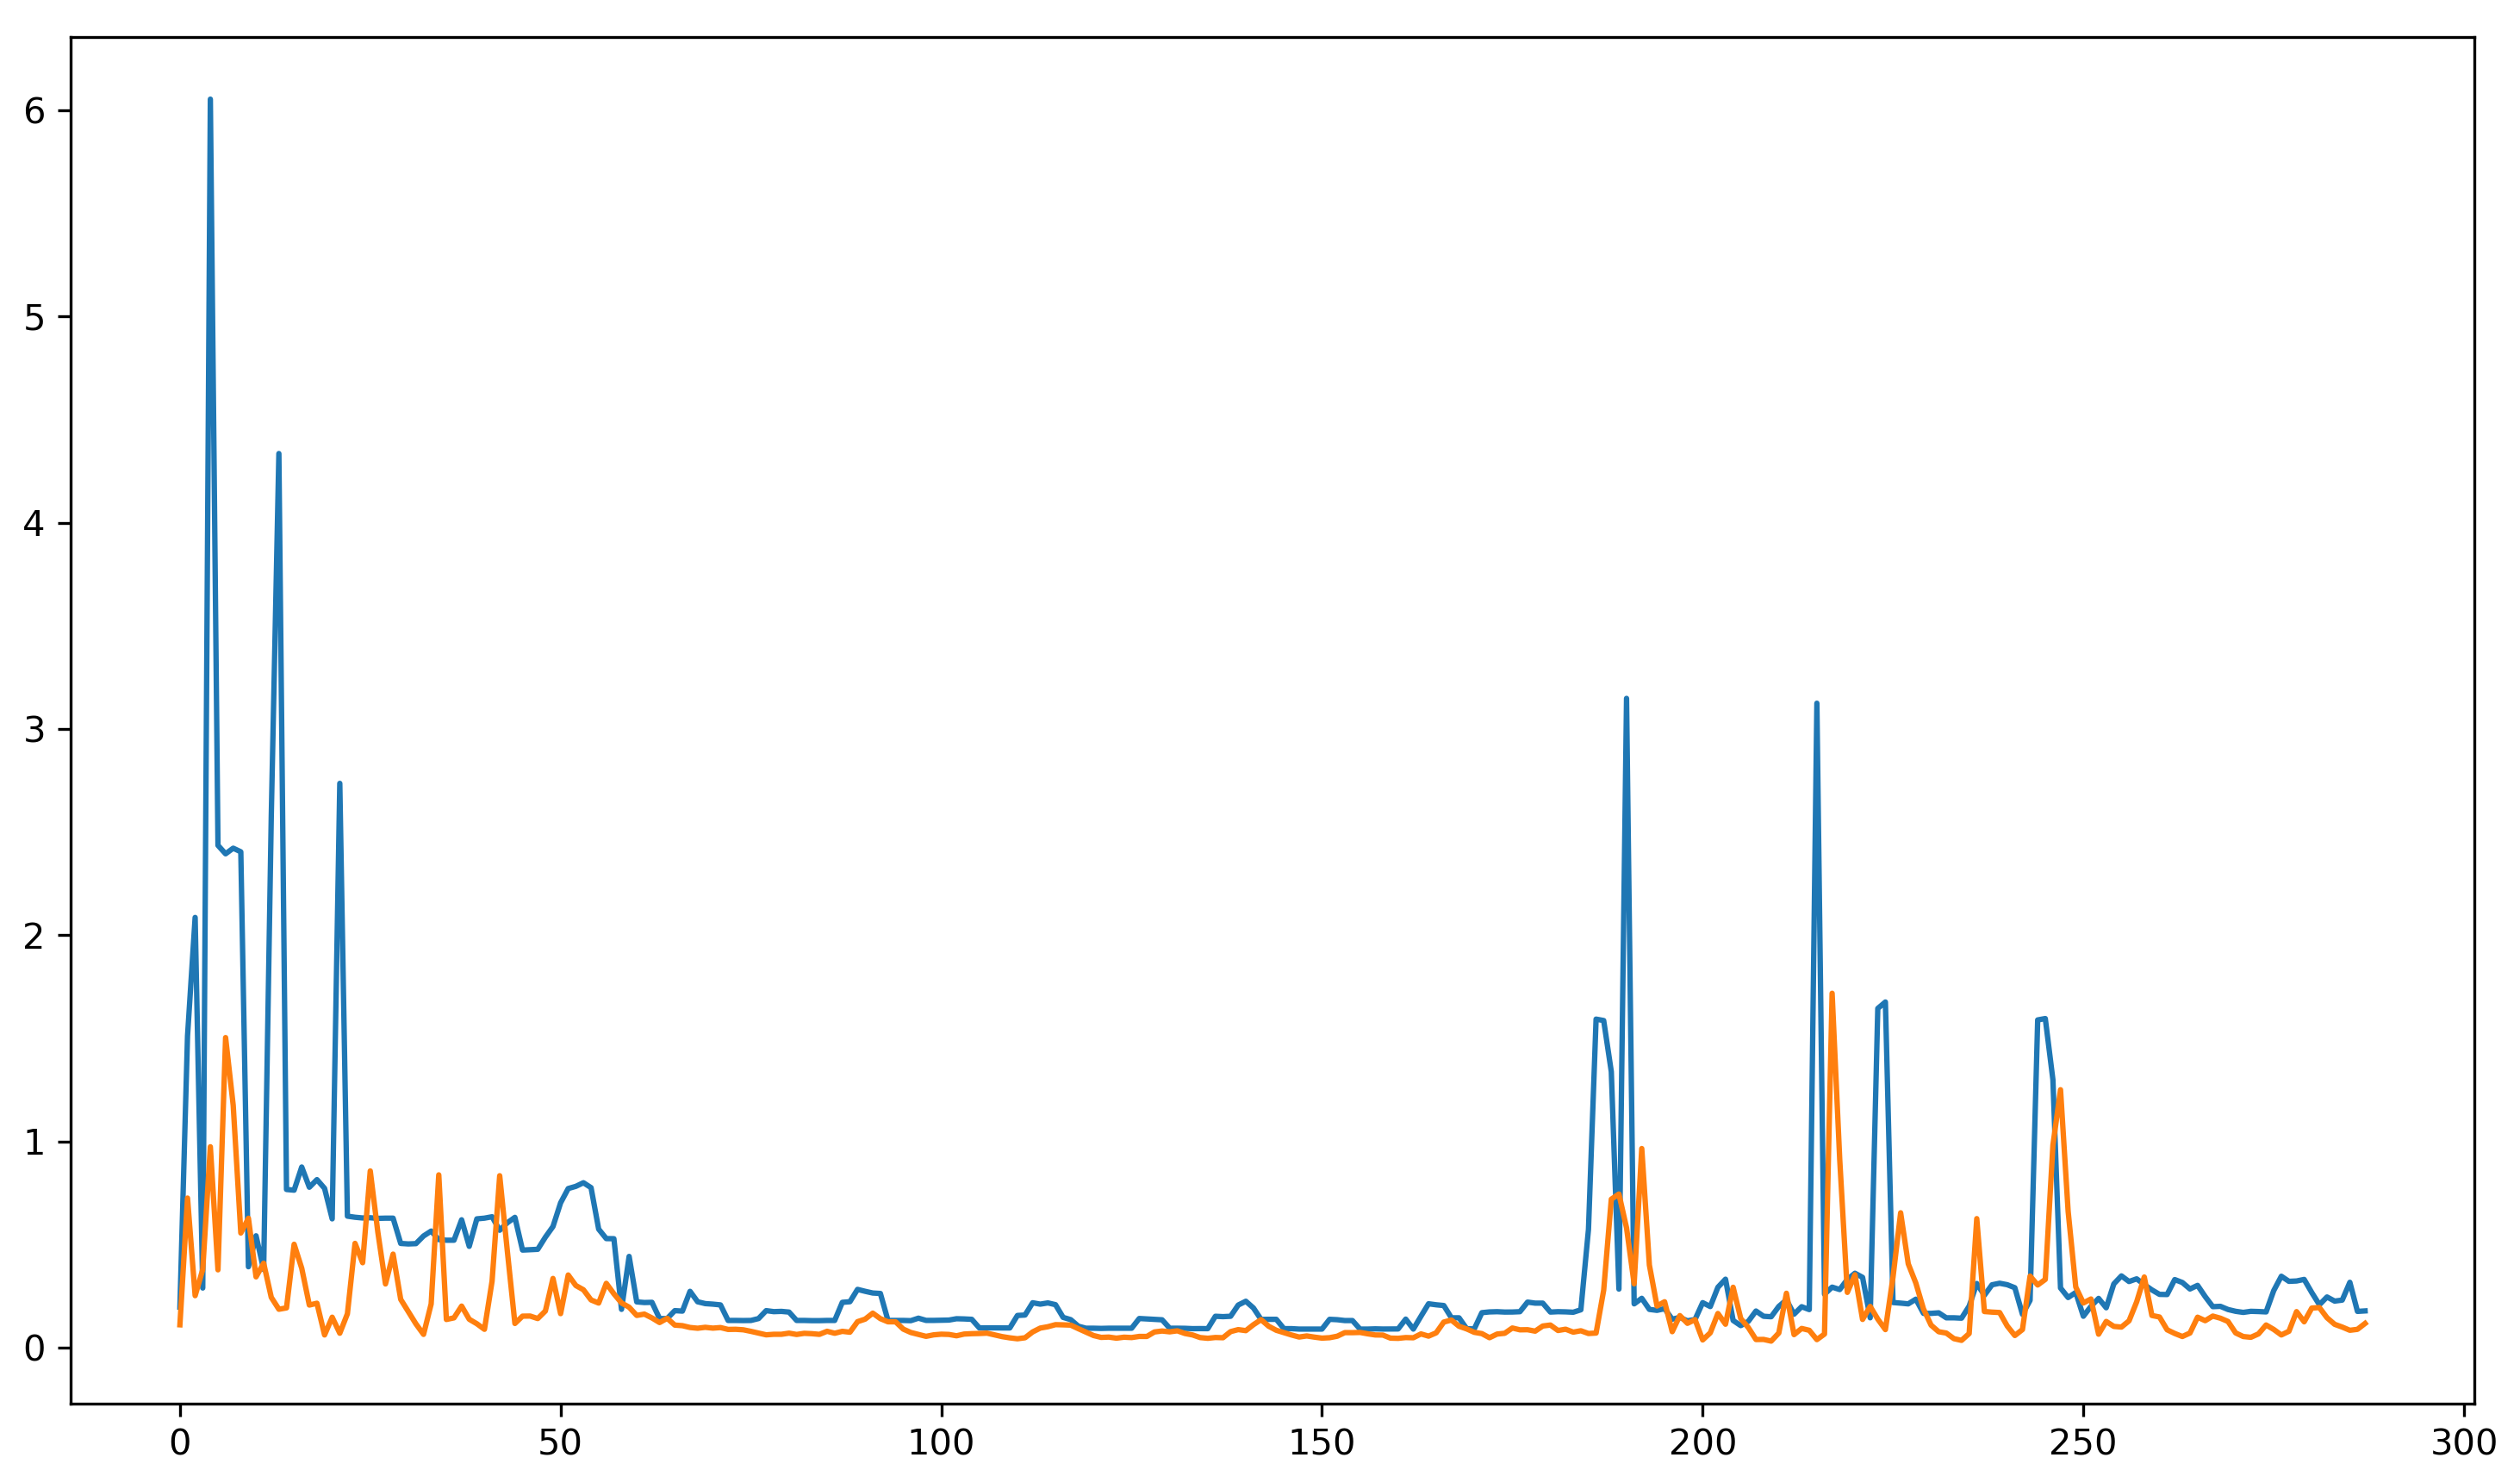
\includegraphics[scale=0.3]{img/c24_test.png}
    \caption{Performance of the model on another building}
    \label{fig:prediction2}
\end{figure}

As mentioned earlier the CNN-LSTM network outperforms other approaches, however, the method needs to be tested on several different datasets and many different architectures (number of neurons, layers, etc.) to accurately analyse the effectiveness of this algorithms in accurate energy demand prediction.

\section*{Conclusion}

This study was conducted to investigated the performance of a CNN-LSTM model for building level energy demand forecasting. The presented model was trained and tested on demand load of a building in Findhorn ecovillage in Scotland and was tested independently on another building in the same area. The proposed model consist of two one dimensional convolutional layer with max pooling, two bidirectional LSTM layers and finally three fully connected dense layer. Furthermore, the performance of the model was tested against ARIMA, RF, LightGBM and a DNN to see if CNN-LSTM show any advantage in this problem. The result was good and the proposed architecture outperformed all well-established models. The RMSE value on the test data was significantly lower that other algorithms. Thus, it can be deduce the CNN-LSTM architecture shows notable potential for accurate load forecasting and it needs to be further studied. For future work, the authors plan to implement a multivariate approach to load forecasting and use a variety of features such as weather related data and building information. In addition, more datasets regarding energy demand forecasting will be collected to train and evaluate the model to achieve even better performance. Furthermore, transfer learning will be study to see its effectiveness on load forecasting.

\section*{Acknowledgement}

The authors would like to acknowledge the Findhorn Foundation and the academic and industry partners within the Centre for Energy Systems Integration (CESI - National Centre for Energy System Integration).

%here starts the references

\bibliographystyle{chicago}
\bibliography{references}

\end{document}
